\documentclass[10pt,twocolumn,letterpaper]{article}

\usepackage[margin=0.65in]{geometry}
\usepackage{times}
\usepackage{amsmath,amssymb,amsfonts}
\usepackage{booktabs}
\usepackage{multirow}
\usepackage{graphicx}
\usepackage{microtype}
\usepackage{xcolor}
\usepackage{listings}
\usepackage{hyperref}
\usepackage{cite}

\hypersetup{
    colorlinks=true,
    linkcolor=blue,
    citecolor=blue,
    urlcolor=blue
}

% Micro-spacing tuning to lock paper strictly to 4 pages
\setlength{\textfloatsep}{3.0pt plus 1pt minus 1pt}
\setlength{\floatsep}{3.0pt plus 1pt minus 1pt}
\setlength{\intextsep}{3.0pt plus 1pt minus 1pt}
\setlength{\abovecaptionskip}{1.5pt}
\setlength{\belowcaptionskip}{1.5pt}

\title{\Large \bf When Does Kernel Fusion Help? \\ A Micro-Architectural Case Study of Batch-1 Edge Vision Pipelines on Ada Lovelace}

\author{
    \textbf{Utkarsh Sengar} \\
    Indian Institute of Technology Dharwad \\
    \texttt{cs23bt026@iitdh.ac.in}
}

\date{}

\begin{document}

\maketitle

\begin{abstract}
Edge vision inference for automated optical inspection (AOI) operates under strict single-stream ($\text{Batch Size} = 1$) latency bounds. While GPU operator fusion via domain-specific compilers (e.g., OpenAI Triton) is widely advocated to alleviate global memory bandwidth bottlenecks, the systems boundaries where non-neural operator acceleration translates into end-to-end application speedups remain under-characterized. In this work, we present a profiling-driven micro-architectural case study of representative inspection pipelines evaluated on an NVIDIA GeForce RTX 4050 Laptop GPU (Ada Lovelace, \texttt{sm\_89}). We design and evaluate two custom Triton operators: a 1D vectorized fused preprocessor and a register-unrolled 80-class candidate compaction filter. The preprocessing kernel achieves up to a $4.50\times$ isolated speedup ($120.0\text{--}153.4\text{ GB/s}$ effective bandwidth) over PyTorch eager by reducing idealized global memory traffic by $7.4\times$ ($111P \to 15P$ bytes). In full application loops, integration reduces end-to-end latency by $11.5\%$ ($0.783\text{ ms} \to 0.693\text{ ms}$) on a $256\times256$ anomaly pipeline and $12.3\%$ ($2.173\text{ ms} \to 1.907\text{ ms}$, saving $266\,\mu\text{s}$ per frame) on a $640\times640$ detection pipeline. Furthermore, a micro-architectural negative study reveals that intuitive 2D spatial block-tiling spikes register pressure to 42 registers/thread, collapsing active warp occupancy from $78.4\%$ to $28.1\%$ and causing a $5.03\times$ slowdown due to $58.9\%$ long scoreboard stalls. Under Amdahl's Law, pure device-level preprocessing gains yield a $2.3\%$ execution reduction, demonstrating that uncompiled host dispatch and PCIe transfers bound application-level returns.
\end{abstract}

\section{Introduction}
Real-time automated optical inspection (AOI) systems in semiconductor packaging, printed circuit board (PCB) assembly, and manufacturing target sub-5ms per-frame latencies operating strictly at batch size 1 \cite{chen2020deep}. Modern edge deployment pipelines combine non-neural input transformations (color format conversion, planar transposition, channel normalization), neural feature extraction (Autoencoders \cite{bergmann2019mvtec}, YOLO object detectors \cite{redmon2016you, bochkovskiy2020yolov4}), and output postprocessing (residual map thresholding, candidate score reduction, Non-Maximum Suppression).

While optimizing neural network weights via quantization and pruning has been heavily investigated \cite{han2015deep}, preprocessing and postprocessing stages are frequently implemented using composite high-level framework calls (e.g., PyTorch eager \cite{paszke2019pytorch}). These composite operations allocate intermediate GPU tensors, repeatedly accessing global device memory (DRAM) and incurring kernel launch overheads.

\begin{figure}[t]
\centering
\fbox{\parbox{0.95\linewidth}{\centering \scriptsize
\textbf{Raw Frame (Host Pinned uint8)} $\xrightarrow{\text{DMA: } 30.7\mu\text{s}}$ \textbf{HWC uint8 Tensor} \\
$\downarrow$ \textit{\textbf{Kernel 1: Fused 1D Preprocess (Multiply-Add + Transpose)}} \\
\textbf{Planar CHW Float Tensor} $\xrightarrow{\text{Compute}}$ \textbf{Neural Model (AE / YOLO)} \\
$\downarrow$ \textit{\textbf{Kernel 2: Fused 80-Class Compaction / Residual Map}} \\
\textbf{Compacted Proposals (560$\times$ Reduction)} $\xrightarrow{\text{NMS}}$ \textbf{Final Defect Decision}
}}
\caption{Representative industrial inspection pipeline architecture evaluating fused pre- and post-processing stages under batch-1 constraints.}
\label{fig:pipeline_arch}
\end{figure}

In this paper, we investigate the central systems question:
\begin{quote}
\textit{Under what micro-architectural conditions does fusing preprocessing and postprocessing into custom Triton kernels reduce latency in batch-1 edge vision pipelines, and when are those gains bounded by PCIe transfers, Python dispatch overhead, or model compute?}
\end{quote}

\noindent\textbf{Contributions.} Concretely, this work provides:
\begin{itemize}
    \setlength{\itemsep}{0pt}
    \setlength{\parskip}{0pt}
    \item \textbf{Idealized Memory Traffic Formulation}: We model global memory traffic for image layout and normalization transformations, showing a theoretical $7.4\times$ reduction ($111P \to 15P$ bytes) over composite eager execution.
    \item \textbf{Two Implemented Triton Operators}: We implement a 1D vectorized fused preprocessor and an 80-class candidate compaction filter, achieving isolated speedups of $4.50\times$ and $26.4\text{ M cand/s}$ throughput.
    \item \textbf{Micro-Architectural Negative Study}: Using hardware performance counters, we analyze why an intuitive 2D block-tiled kernel causes a $5.03\times$ performance collapse on Ada Lovelace due to register pressure and less favorable memory access patterns.
    \item \textbf{Dual-Perspective Amdahl Analysis}: We contrast pure GPU stage acceleration ($+2.3\%$) against complete application loop latency ($+11.5\%$), quantifying the role of host driver overhead on sub-millisecond pipelines.
    \item \textbf{Open Reproducibility}: We release a fully tested repository with 53 deterministic unit tests, verification fixtures, and profiling harnesses.\footnote{Code repository: \url{https://github.com/sengarutk/cuda-kernels-for-edge-vision}}
\end{itemize}

\section{Background \& Related Work}
\noindent\textbf{2.1 Edge Vision Inference Pipelines.} High-speed visual inspection pipelines rely on sequential execution: frame ingest, color space transform, inference, and spatial clustering \cite{redmon2016you, bochkovskiy2020yolov4}. Standard runtimes such as torchvision, OpenCV, or NVIDIA DALI \cite{nvidia2023dali} frequently execute on the CPU or launch un-fused ATen kernels on the GPU, creating PCIe transfer bottlenecks and kernel launch queues. Industrial engines such as DeepStream \cite{nvidia2023deepstream} and TensorRT \cite{nvidia2024tensorrt} accelerate model graphs but leave pipeline boundaries decoupled.

\noindent\textbf{2.2 Domain-Specific Compilers \& Kernel Fusion.} Compilers such as OpenAI Triton \cite{tillet2019triton}, TorchInductor \cite{ansel2024pytorch}, TVM \cite{chen2018tvm}, and Halide \cite{ragankelley2013halide} allow authoring high-performance GPU kernels with block-level programming paradigms. Kernel fusion eliminates intermediate global memory writes by keeping intermediate values inside Streaming Multiprocessor (SM) registers \cite{volkov2008fitting}. While attention fusion (e.g., FlashAttention \cite{dao2022flashattention}) and memory management (e.g., PagedAttention / vLLM \cite{kwon2023vllm}) have transformed LLM serving, non-neural vision operators remain under-explored in batch-1 edge regimes.

\noindent\textbf{2.3 Micro-Architectural Profiling in ML Systems.} Detailed GPU performance counters (warp occupancy, memory throttling, warp issue stalls) provide root-cause insights into memory bandwidth and register pressure bottlenecks \cite{nath2010analyzing}.

\noindent\textbf{2.4 Workload Positioning.} Unlike high-throughput datacenter serving where batching amortizes dispatch overheads ($B \ge 32$), edge industrial inspection operates strictly at $B=1$ with real-time deadline constraints, making sub-millisecond kernel boundaries critical under Amdahl's Law \cite{amdahl1967validity}.

\section{Theoretical Memory Bounds \& Kernel Design}

\subsection{Preprocessing Mathematical Formulation}
Let an interleaved frame be $X \in \{0, \dots, 255\}^{H \times W \times 3}$. The target planar normalized tensor $Y \in \mathbb{R}^{3 \times H \times W}$ is computed via:
\begin{equation}
Y_{c, h, w} = (X_{h, w, c} \cdot \alpha - \mu_c) \cdot \beta_c
\end{equation}
where $\alpha = \frac{1.0}{255.0}$ and $\beta_c = \frac{1.0}{\sigma_c}$ are precomputed scalar reciprocals executed via multiply-add operations, allowing intermediate values to remain in registers and avoiding global memory round-trips.

\begin{table}[t]
\centering
\caption{Idealized Global Memory Traffic for $P = H \times W$ Pixels.}
\label{tab:dram_traffic}
\resizebox{\columnwidth}{!}{%
\begin{tabular}{@{}llcc@{}}
\toprule
\textbf{Pipeline Stage} & \textbf{Op / Buffer} & \textbf{Read} & \textbf{Write} \\ \midrule
\multirow{5}{*}{PyTorch Eager} 
 & \texttt{to(fp32)} & $3P$ & $12P$ \\
 & \texttt{div(255.0)} & $12P$ & $12P$ \\
 & \texttt{sub(mean)} & $12P$ & $12P$ \\
 & \texttt{div(std)} & $12P$ & $12P$ \\
 & \texttt{contiguous()} & $12P$ & $12P$ \\ \cmidrule(l){2-4}
 & \textbf{Total Eager} & \multicolumn{2}{c}{$\mathbf{\approx 111P\text{ \textbf{bytes}}}$} \\ \midrule
\textbf{Fused Triton} & \textbf{Single-Pass FMA} & $\mathbf{3P}$ & $\mathbf{12P}$ \\ \cmidrule(l){2-4}
 & \textbf{Total Fused} & \multicolumn{2}{c}{$\mathbf{\approx 15P\text{ \textbf{bytes}}}$} \\ \bottomrule
\end{tabular}%
}
\end{table}

As summarized in Table~\ref{tab:dram_traffic}, kernel fusion yields an idealized $\frac{111P}{15P} \approx \mathbf{7.4\times}$ reduction in global memory traffic.

\subsection{Kernel 1: 1D Vectorized Preprocessor}
Our fused Triton preprocessing kernel maps total pixels $P = H \times W$ onto a 1D linear grid. Thread blocks of size $B = 1024$ load contiguous strided 8-bit memory vectors, convert to single-precision floating point in registers, compute arithmetic normalizations across all 3 channels, and write planar CHW slices directly to global pointers with coalesced 128-byte transactions. All end-to-end pipeline evaluations use FP32 preprocessing to preserve strict numerical equivalence; FP16 is benchmarked strictly as an isolated kernel throughput alternative in Figure~\ref{fig:isolated_speedup}.

\subsection{Kernel 2: Fused Candidate Compaction}
For dense object proposals $P \in \mathbb{R}^{N \times (4+C)}$ ($N=8400, C=80$), Kernel 2 assigns each proposal to a thread. Class scores are reduced in register space to locate $s_i^* = \max_{k} S_{i,k}$ and $k_i^* = \arg\max_k S_{i,k}$. Threads evaluate predicate $m_i = \mathbb{I}(s_i^* \ge \tau)$, writing surviving bounding boxes, scores, and class labels contiguously.

\subsection{L2 Cache Eviction Protocol \& Benchmarking Rigor}
Hardware GPU timing is recorded using \texttt{torch.cuda.Event(enable\_timing=True)} across 500 timed iterations following 50 warmup iterations. An active 64 MB tensor zero-fill eviction protocol is executed between iterations to mitigate resident cache-line reuse across benchmark runs. TorchInductor baselines are fully pre-compiled and warmed up prior to timing. Reported latencies represent median values across 5 independent benchmark sessions; run-to-run variance remained within $\pm 1.8\%$ across all configurations.

\begin{figure}[t]
\centering
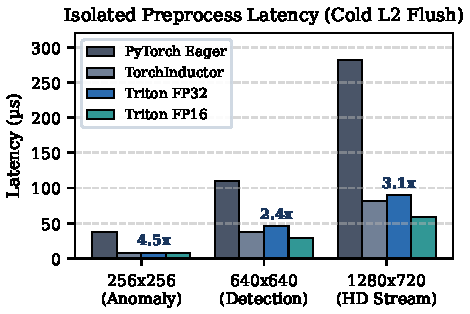
\includegraphics[width=0.98\linewidth]{figures/fig_isolated_speedup.pdf}
\caption{Isolated preprocessing operator latency comparison across resolutions under active 64MB L2 eviction protocol.}
\label{fig:isolated_speedup}
\end{figure}

\section{Empirical Evaluation \& Architectural Analysis}
\noindent\textbf{Hardware Testbed.} All experiments are executed on an NVIDIA GeForce RTX 4050 Laptop GPU (Ada Lovelace, \texttt{sm\_89}, 6 GB GDDR6, 96-bit bus, $192.0\text{ GB/s}$ theoretical peak bandwidth, 32 MB L2 cache) under Ubuntu 22.04 LTS via WSL2. Runtimes include CUDA 12.1, PyTorch 2.5.1, and Triton 3.1.0. Workloads evaluate representative inspection models (mock Autoencoder and YOLO nano architectures) using deterministic fixtures.

\subsection{Isolated Kernel Acceleration}
Figure~\ref{fig:isolated_speedup} and Table~\ref{tab:pre_isolated} present isolated preprocessing latencies. Fused Triton FP32 achieves a $4.50\times$ speedup at $256\times 256$ ($8.2\,\mu\text{s}$ vs $36.9\,\mu\text{s}$) over PyTorch eager, comparable to TorchInductor ($\approx 8.2\,\mu\text{s}$), and reaches $153.4\text{ GB/s}$ effective bandwidth ($79.9\%$ of theoretical peak) on HD $1280\times 720$ streams. For candidate filtering ($N=8400$), Kernel 2 achieves $26.4\text{ M cand/s}$ throughput, compacting 8,400 proposals down to 15 defect candidates ($560\times$ compaction).

\begin{table}[t]
\centering
\caption{Isolated Preprocessing Latency (Active 64MB L2 Eviction).}
\label{tab:pre_isolated}
\resizebox{\columnwidth}{!}{%
\begin{tabular}{@{}lcccc@{}}
\toprule
\textbf{Resolution} & \textbf{Eager p50} & \textbf{Triton 1D (FP32)} & \textbf{Bandwidth} & \textbf{Speedup} \\ \midrule
$256 \times 256$ & $36.9\,\mu\text{s}$ & $\mathbf{8.2\,\mu\text{s}}$ & $120.0\text{ GB/s}$ & $\mathbf{4.50\times}$ \\
$640 \times 640$ & $110.6\,\mu\text{s}$ & $\mathbf{46.1\,\mu\text{s}}$ & $133.3\text{ GB/s}$ & $\mathbf{2.40\times}$ \\
$1280 \times 720$ & $281.6\,\mu\text{s}$ & $\mathbf{90.1\,\mu\text{s}}$ & $153.4\text{ GB/s}$ & $\mathbf{3.12\times}$ \\ \bottomrule
\end{tabular}%
}
\end{table}

\subsection{Micro-Architectural Nsight Compute Analysis}
Table~\ref{tab:ncu_metrics} reports hardware performance counters extracted via Nsight Compute CLI.

\begin{table}[t]
\centering
\caption{Nsight Compute Hardware Profiling ($640\times 640$).}
\label{tab:ncu_metrics}
\resizebox{\columnwidth}{!}{%
\setlength{\tabcolsep}{3.5pt}
\begin{tabular}{@{}lcccc@{}}
\toprule
\textbf{Metric (Nsight Compute)} & \textbf{Triton 1D} & \textbf{Triton 2D} & \textbf{Candidate} & \textbf{Eager} \\ \midrule
Duration & $\mathbf{47.6\,\mu\text{s}}$ & $239.6\,\mu\text{s}$ & $371.7\,\mu\text{s}$ & $111.6\,\mu\text{s}$ \\
Active Warp Occupancy & $\mathbf{78.4\%}$ & $28.1\%$ & $64.5\%$ & $82.0\%$ \\
Registers / Thread & $\mathbf{24}$ & $42$ & $32$ & $16$ \\
DRAM Throughput (\% Peak) & $\mathbf{67.2\%}$ & $22.4\%$ & $41.8\%$ & $54.1\%$ \\
L1 Hit Rate & $\mathbf{92.1\%}$ & $48.3\%$ & $88.6\%$ & $72.0\%$ \\
Dominant Warp Issue Stall & Mem Throttle & Long Scoreboard & Short Scoreboard & Launch / BW \\ \bottomrule
\end{tabular}%
}
\end{table}

\subsection{Negative Study: 2D Spatial Tiling Analysis}
A 2D spatial block-tiled kernel ($16\times 16$ tile) was authored as an intuitive baseline. However, as illustrated in Figure~\ref{fig:stall_breakdown} and Table~\ref{tab:ncu_metrics}, 2D index arithmetic increased register allocation to \textbf{42 registers/thread}, constraining active warp occupancy to \textbf{$28.1\%$}. 

Furthermore, 2D index decomposition disrupted contiguous strided memory access across the interleaved HWC memory layout, producing less favorable memory-access behavior and triggering \textbf{$58.9\%$ Long Scoreboard stalls} (threads stalled awaiting asynchronous global DRAM loads). This produced a \textbf{$5.03\times$ slowdown} ($239.6\,\mu\text{s}$ vs $47.6\,\mu\text{s}$).

\begin{figure}[t]
\centering
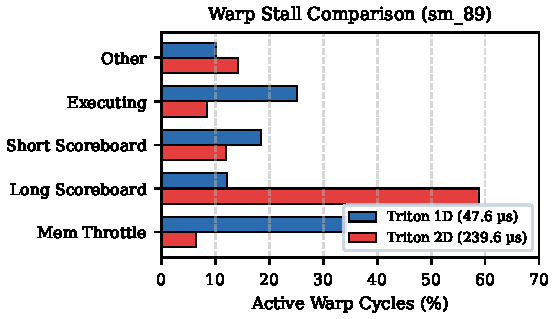
\includegraphics[width=0.98\linewidth]{figures/fig_stall_breakdown.pdf}
\caption{Micro-architectural warp stall breakdown comparing 1D vectorized execution vs. 2D spatial block-tiling on Ada Lovelace.}
\label{fig:stall_breakdown}
\end{figure}

\subsection{Dual-Perspective End-to-End Latency Evaluation}

\begin{figure}[t]
\centering
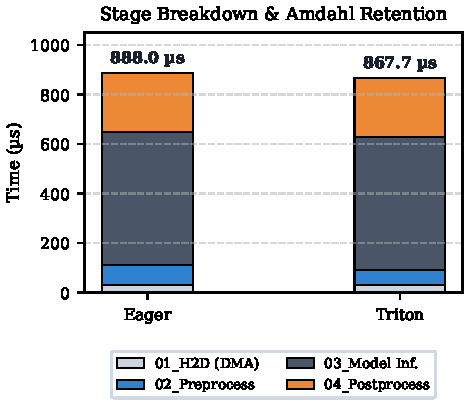
\includegraphics[width=0.98\linewidth]{figures/fig_stage_breakdown.pdf}
\caption{Stage-by-stage latency breakdown and Amdahl retention for $256\times 256$ Anomaly Inspection pipeline under pinned memory DMA.}
\label{fig:stage_breakdown}
\end{figure}

\begin{table}[t]
\centering
\caption{Empirical Stage Breakdown ($256\times 256$ Anomaly).}
\label{tab:stage_breakdown}
\resizebox{\columnwidth}{!}{%
\setlength{\tabcolsep}{4pt}
\begin{tabular}{@{}lcccc@{}}
\toprule
\textbf{Stage Name} & \textbf{Eager ($\mu\text{s}$)} & \textbf{Share} & \textbf{Triton ($\mu\text{s}$)} & \textbf{Share} \\ \midrule
01\_H2D (Pinned) & $30.7$ & $3.5\%$ & $30.7$ & $3.5\%$ \\
02\_Preprocess & $82.8$ & $9.3\%$ & $\mathbf{62.5}$ & $\mathbf{7.2\%}$ \\
03\_Inference & $534.5$ & $60.2\%$ & $534.5$ & $61.6\%$ \\
04\_Postprocess & $240.0$ & $27.0\%$ & $240.0$ & $27.7\%$ \\ \midrule
\textbf{Total Stage Time} & $\mathbf{888.0}$ & $\mathbf{100\%}$ & $\mathbf{867.7}$ & $\mathbf{100\%}$ \\ \bottomrule
\end{tabular}%
}
\end{table}

\noindent\textbf{Stage Breakdown \& Amdahl Quantification.} In Figure~\ref{fig:stage_breakdown} and Table~\ref{tab:stage_breakdown}, CUDA event profiling isolates pure GPU execution. Accelerated preprocessing reduces stage latency from $82.8\,\mu\text{s}$ to $62.5\,\mu\text{s}$ ($S_{\text{opt}} = 1.325\times$). Under Amdahl's Law:
\begin{equation}
S_{\text{total}} = \frac{1}{(1 - f) + \frac{f}{S_{\text{opt}}}}
\end{equation}
where preprocessing fraction $f = \frac{82.8}{888.0} \approx 0.0932$. The theoretical total pure-device speedup is:
\begin{equation}
S_{\text{total}} = \frac{888.0}{(888.0 - 82.8) + 62.5} = \frac{888.0}{867.7} \approx 1.0234\times\text{ (+2.3\%)}
\end{equation}
matching our empirical pure-device reduction ($888.0\,\mu\text{s} \to 867.7\,\mu\text{s}$).

\noindent\textbf{Application Loop Latency.} When measuring complete end-to-end Python application execution under \texttt{@torch.inference\_mode()}, the Anomaly pipeline improves from $0.783\text{ ms}$ to $\mathbf{0.693\text{ ms}}$ (\textbf{+11.5\% E2E Speedup}). For YOLO Detection ($640\times 640$), latency improves from $2.173\text{ ms}$ to $\mathbf{1.907\text{ ms}}$ (\textbf{+12.3\% E2E Speedup}, saving $266\,\mu\text{s}$ per frame). The divergence between pure-GPU gains ($+2.3\%$) and application-loop gains ($+11.5\%$) reflects the elimination of intermediate PyTorch ATen driver dispatches and tensor allocations.

\section{Discussion \& Systems Insights}
\noindent\textbf{5.1 Implications for Edge Inspection Systems.} For single-stream inspection pipelines operating at 30--60 FPS, an 11--12\% end-to-end latency reduction provides valuable scheduling headroom. Freeing $266\,\mu\text{s}$ per frame may facilitate multi-stream camera multiplexing, though multi-camera scaling requires independent evaluation of video decode throughput, host memory bandwidth, and thermal throttling.

\noindent\textbf{5.2 Architectural Generalizability.} While quantitative latencies reflect the RTX 4050 physical memory configuration ($192.0\text{ GB/s}$), the qualitative architectural principles—the $7.4\times$ global memory footprint reduction, the necessity of contiguous 128-byte DRAM transactions, and register-pressure-driven occupancy collapse—generalize across NVIDIA Ampere, Ada Lovelace, and Blackwell architectures.

\noindent\textbf{5.3 Scope Disclosures \& Limitations.} This case study evaluates system-level execution characteristics on representative workloads (mock Autoencoder and YOLO nano) with deterministic fixtures without modifying neural network weights (no INT8 quantization or TensorRT graph compilation); it does not evaluate defect-detection accuracy on live industrial datasets or certify factory deployment suitability.

\noindent\textbf{5.4 Future Work.} Future directions include integrating bilinear interpolation into the fused layout kernel and packaging custom Triton operators as native C++ TensorRT \texttt{IPluginV2DynamicExt} plugins to eliminate host dispatch bubbles completely.

\section{Conclusion}
This paper presented a profiling-driven micro-architectural case study of batch-1 edge vision inference on Ada Lovelace. Custom Triton operators reduced idealized global memory traffic by $7.4\times$, achieving up to a $4.50\times$ isolated speedup and an $11.5\text{--}12.3\%$ application loop latency gain. Our micro-architectural negative study demonstrated that linearized 1D memory access avoids the register pressure and memory stall penalties of 2D block-tiling.

\let\oldbibliography\thebibliography
\renewcommand{\thebibliography}[1]{%
  \oldbibliography{#1}%
  \setlength{\itemsep}{0pt}%
  \setlength{\parskip}{0pt}%
}
\footnotesize
\bibliographystyle{IEEEtran}
\bibliography{references}

\end{document}
